\subsection{Unconditional Image Generation}

We evaluate our method on the task of unconditional image generation on datasets
FFHQ256, FFHQ1024, CelebA, LSUN Churches, and LSUN Bedrooms. For LSUN we use
pretrained \gls{vqgan} checkpoints provided by~\cite{bondtaylor2021unleashing},
and for all other unconditional experiments we use checkpoints from the original
work~\cite{esser2021taming}. We evaluate in terms of raw perceptual quality and
coverage, as well as how these metrics are affected by the various
hyperparameters of our model and parameters of the sampling process -- the
latter of which we found to be highly configurable.

\begin{figure}[ht]
    \centering
    \begin{subfigure}[b]{\textwidth}
        \centering
        \includegraphics[width=1.0\textwidth]{figures/ffhq256-samples.png}
        \caption{
            Multiple outputs of inpainting on the same block mask. Multiple
            realistic results are produced at a very high resolution.
        }
    \end{subfigure}
    %\hfill
    %\begin{subfigure}[b]{0.47\textwidth}
        %\centering
        %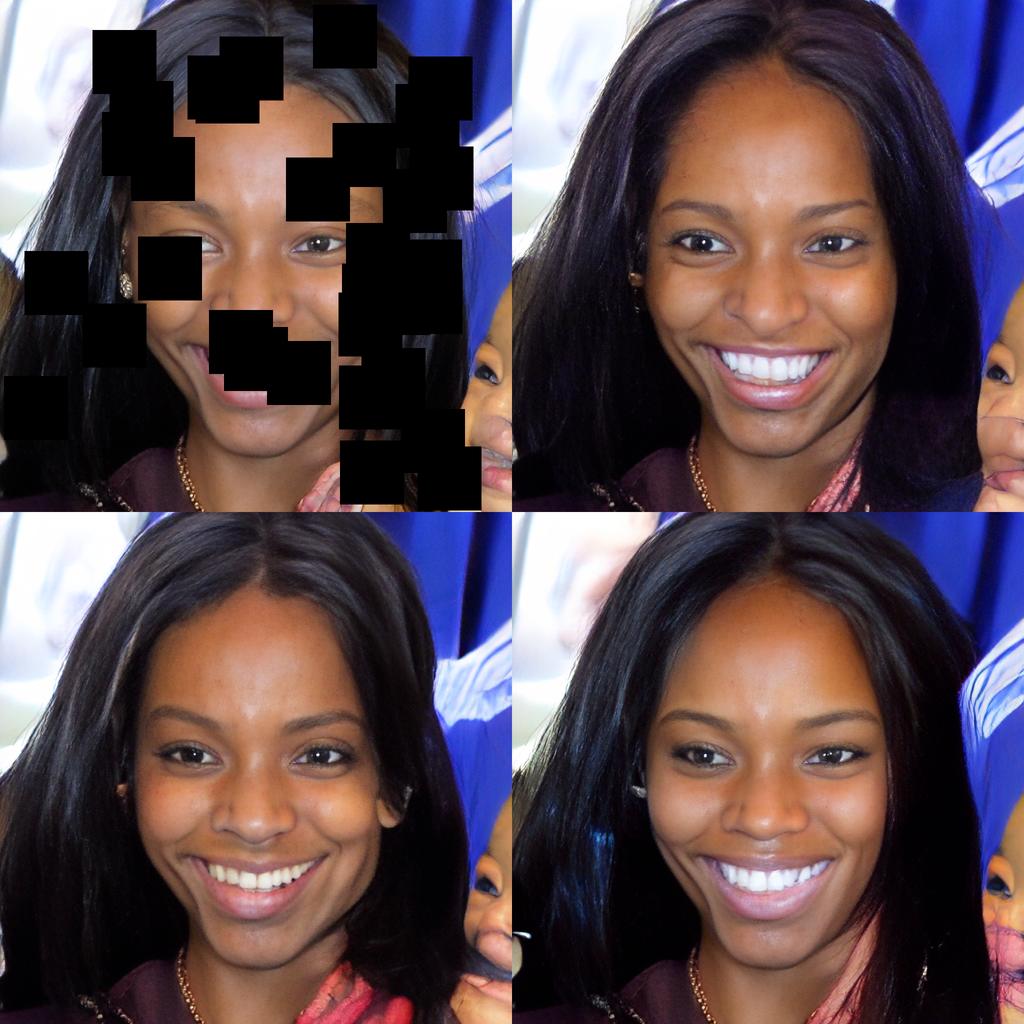
\includegraphics[width=1.0\textwidth]{figures/inpaint-rand/inpaint-variation-small.png}
        %\caption{
            %Multiple outputs of inpainting on the same random mask. Multiple
            %realistic results are produced at a very high resolution.
        %}
    %\end{subfigure}
    %\caption{Inpainting results on FFHQ-1024.}
\end{figure}

\subsection{Conditional Image Generation}

\begin{figure}[ht]
    \centering
    \begin{subfigure}[b]{0.47\textwidth}
        \centering
        \includegraphics[width=1.0\textwidth]{figures/mnist-samples.png}
        \caption{
            Conditional, pixel-wise generation on MNIST.
        }
    \end{subfigure}
    \hfill
    \begin{subfigure}[b]{0.47\textwidth}
        \centering
        \includegraphics[width=1.0\textwidth]{figures/fashionmnist-samples.png}
        \caption{
            Conditional, pixel-wise generation on Fashion-MNIST.
        }
    \end{subfigure}
    \caption{Testing conditional generation using MNIST-style datasets.}
\end{figure}

Another critical component of an ideal generative model is the ability to
control its generation. We explore class-conditioned image generation of
ImageNet at $256 \times 256$ resolution, using the pretrained ImageNet
\gls{vqgan} checkpoints provided by the original work~\cite{esser2021taming}. To
introduce class information to the model, we add an additional embedding layer
(one embedding for each of the 1000 classes) and add this to all input token
embeddings, as done in Image Transformer~\cite{parmar2018image}. We again,
perform our evaluation using metrics of perceptual quality and distribution
coverage.

\subsection{Arbitrary Image Inpainting}

As outlined earlier, \acrlong{nar} generative models have a number of advantages
on inpainting tasks, including supporting arbitrary masks and being able to use
the full context available to them. We provide a number of examples of
inpainting on FFHQ1024 and ImageNet, showcasing different patterns and different
results given the same starting image. As our method utilises a vector quantized
image model, it is incapable of doing fine-grained inpainting at a pixel level.
Nonetheless, the results show consistently good inpainting results when
operating at a \gls{vq} latent level.

\begin{figure}[ht]
    \centering
    \begin{subfigure}[b]{\textwidth}
        \centering
        \label{fig:inpaintExample}
        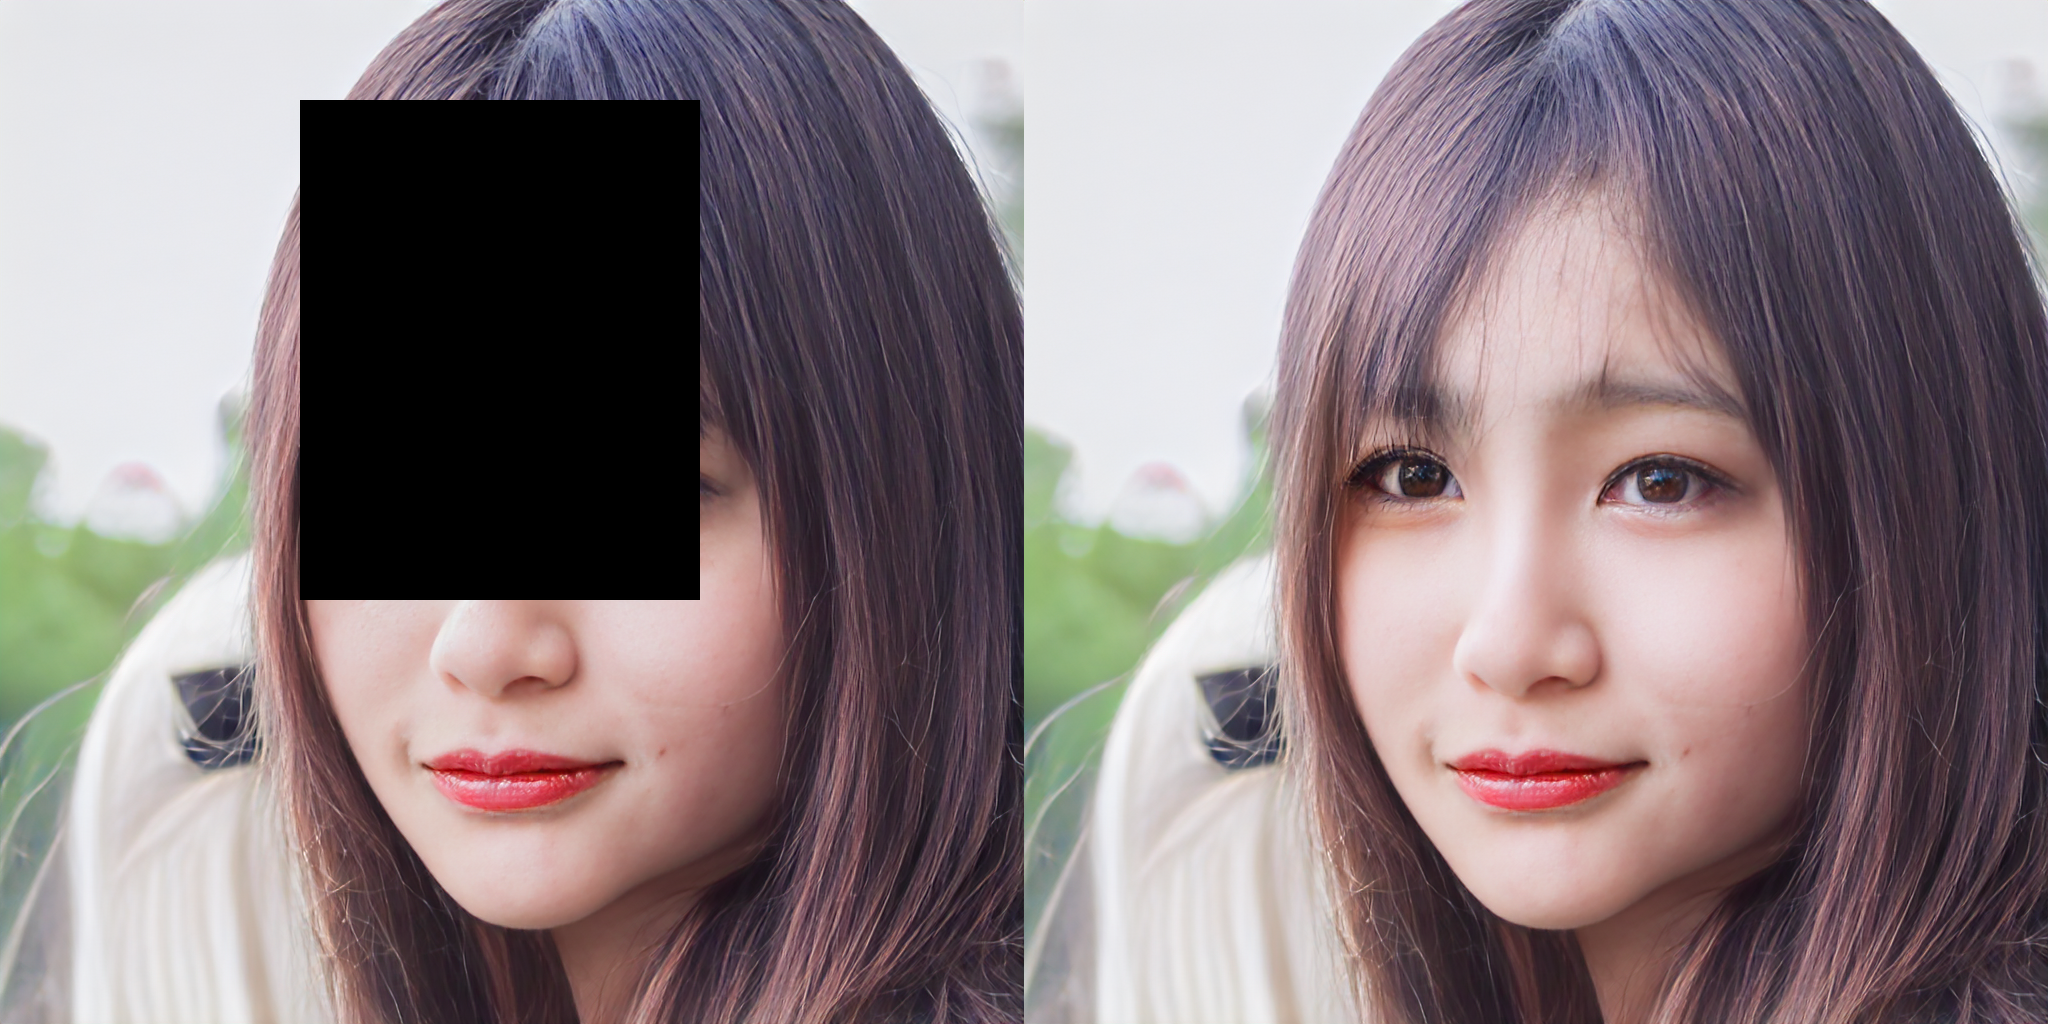
\includegraphics[width=1.0\linewidth]{figures/inpaint.png}
        \caption{A large example of inpainting on a $1024 \times 1024$ image using our
        model.}
    \end{subfigure}
    \\
    \begin{subfigure}[b]{0.47\textwidth}
        \centering
        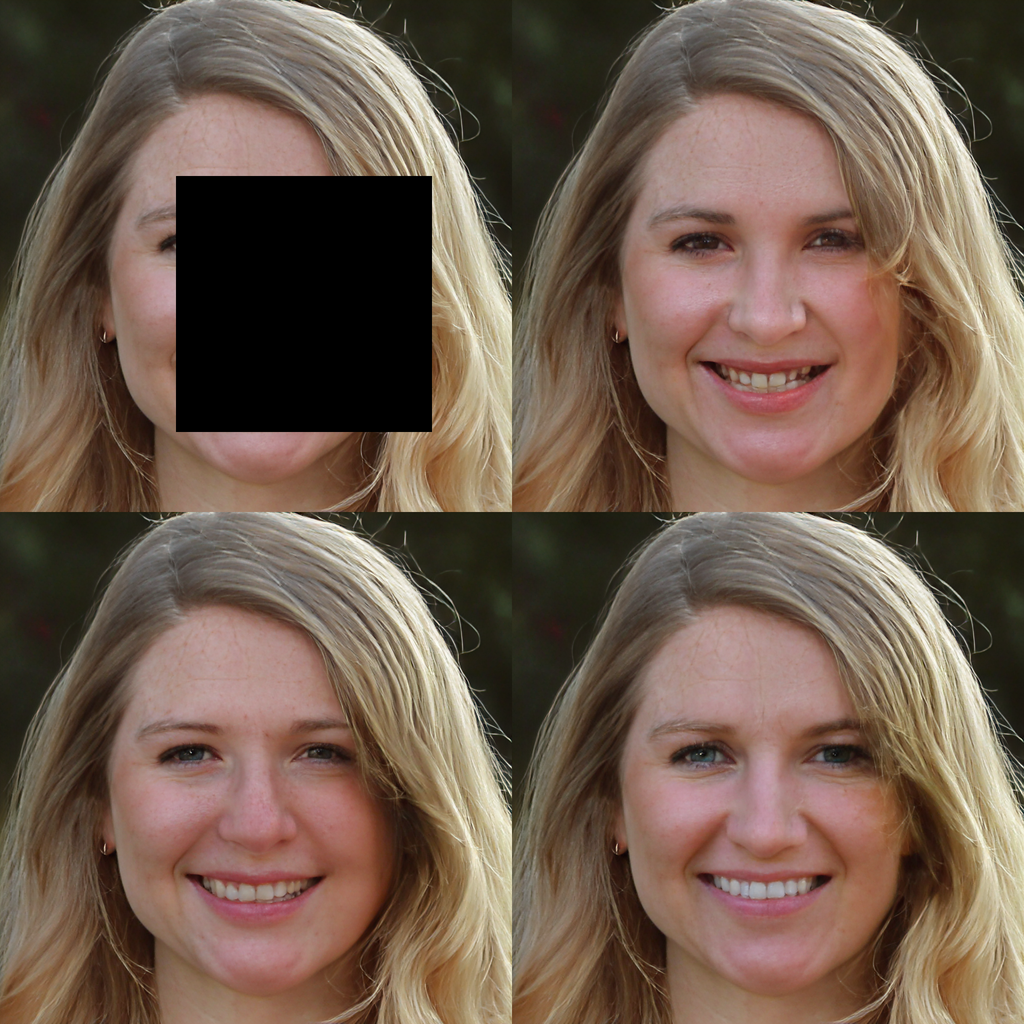
\includegraphics[width=1.0\textwidth]{figures/inpaint-block/inpaint-variation-small.png}
        \caption{
            Multiple outputs of inpainting on the same block mask. Multiple
            realistic results are produced at a very high resolution.
        }
    \end{subfigure}
    \hfill
    \begin{subfigure}[b]{0.47\textwidth}
        \centering
        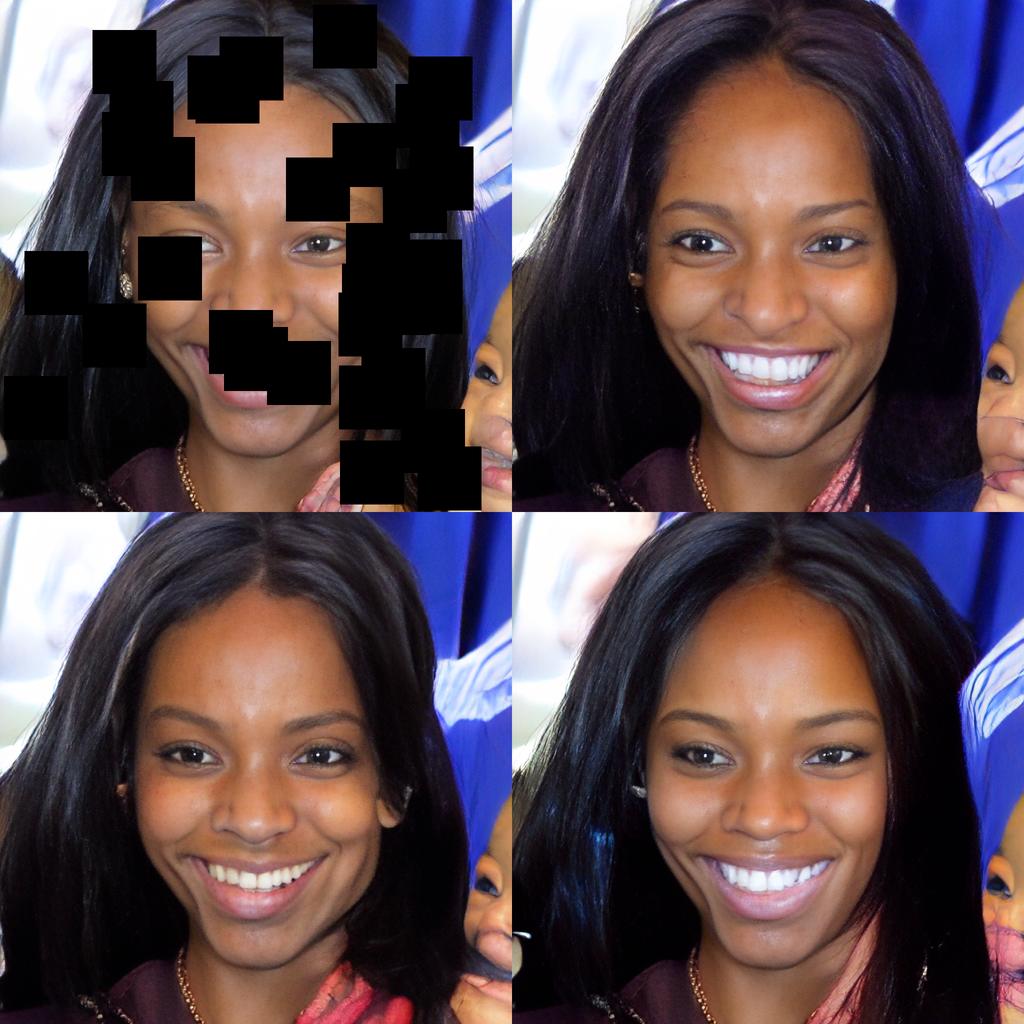
\includegraphics[width=1.0\textwidth]{figures/inpaint-rand/inpaint-variation-small.png}
        \caption{
            Multiple outputs of inpainting on the same random mask. Multiple
            realistic results are produced at a very high resolution.
        }
    \end{subfigure}
    \caption{Inpainting results on FFHQ-1024.}
\end{figure}

